\hypertarget{simulation}{%
\section{Simulation}\label{simulation}}

\hypertarget{simulation-modeling}{%
\subsection{Simulation = Modeling}\label{simulation-modeling}}

It's not possible to simulate something without a model.

Definition Modeling:\\
Deriving calculation schemes (models) where the output variables can
predicted sufficiently accurately from the input variables.

\hypertarget{finding-a-model}{%
\subsubsection{Finding a model}\label{finding-a-model}}

One way is to play with the real system to find out how it works and
reacts. If this is possible and the possible damage is low, it might be
a good idea. If the damage is big, it is better to recreate a physical
model (e.g.~a big pool to simulate a lake.)

\begin{figure}
\centering
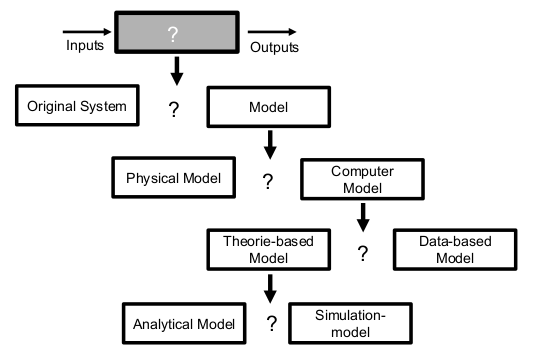
\includegraphics{figures/system_analysis_landscape.png}
\caption{system analysis landscape}
\end{figure}

\hypertarget{different-simulation-paradigms}{%
\subsection{Different simulation
paradigms}\label{different-simulation-paradigms}}

\hypertarget{monte-carlo-simulation}{%
\subsubsection{Monte Carlo Simulation}\label{monte-carlo-simulation}}

MC Simulation is a broad class of algorithms that rely on repeated
sampling to obtain numerical results.

\hypertarget{system-dynamics}{%
\subsubsection{System Dynamics}\label{system-dynamics}}

SD is an approach for understanding the behavior of complex systems over
time, using stocks, flows, feedback loops, and time delays.

\hypertarget{discrete-event-simulation}{%
\subsubsection{Discrete Event
Simulation}\label{discrete-event-simulation}}

Simulation, where system state only changes at discrete points in time.
Key element: Queue.

\hypertarget{multi-agend-simulation}{%
\subsubsection{Multi-agend Simulation}\label{multi-agend-simulation}}

In MA Simulation, we have a system that consists of multiple entities
with identical or different behavior. They solve problems collectively.

\hypertarget{monte-carlo-simulation-1}{%
\section{Monte Carlo Simulation}\label{monte-carlo-simulation-1}}

MC Simulation is a numerical method for statistical simulation. It is
based on using sequences of random numbers in order to explore the
behavior of the system. Monte-Carlo simulation also provides an
alternative for solving complex problems in probability and statistics.

\hypertarget{monte-carlo-model}{%
\subsection{Monte Carlo Model}\label{monte-carlo-model}}

\begin{figure}
\centering
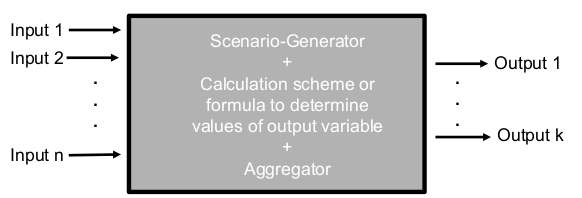
\includegraphics{figures/montecarloModel.png}
\caption{Monte Carlo Model}
\end{figure}

\begin{enumerate}
\def\labelenumi{\arabic{enumi}.}
\tightlist
\item
  The Scenario-Generator creates scenarios according to a prescribed
  probability distributions that match reality.
\item
  Each scenario yields values of the target variable that can be
  obtained via a calculation scheme or formula.
\item
  The Aggregator calculates the output(s) form the target values
  associated with each simulated scenario.
\end{enumerate}

\hypertarget{discrete-event-simulation-1}{%
\section{Discrete Event Simulation}\label{discrete-event-simulation-1}}

A Simulation-model is a virtual representation of a real-world system
that allows to gain insights in how the system works in reality.

\hypertarget{queuing-system}{%
\subsection{Queuing System}\label{queuing-system}}

In a queuing system, \textbf{jobs} are processed by a \textbf{server}.
Under the (realistic) assumption that the server has a particular
limited capacity (e.g.~specified as the maximum number of jobs that can
processed per hour), the system can get congested and waiting times may
occur.

\hypertarget{advantages}{%
\subsection{Advantages}\label{advantages}}

\begin{itemize}
\tightlist
\item
  Cost-effective, fast, and safe field of experimentation (compared to
  experimenting with original system)
\item
  Allows animation and hence increases system understanding
\item
  Allows the analysis of complex systems at a high level of detail
  (compared to analytical solutions)
\end{itemize}

\hypertarget{disadvantages}{%
\subsection{Disadvantages}\label{disadvantages}}

\begin{itemize}
\tightlist
\item
  Requires significant (software) development time
\item
  Construction of a simulation model is relatively prone to error
\item
  Sound interpretation of results is challenging
\end{itemize}

\begin{figure}
\centering
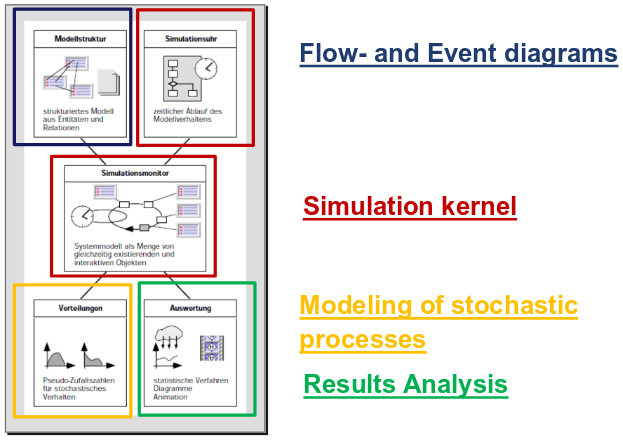
\includegraphics{figures/overviewDES.png}
\caption{Overview DES}
\end{figure}

\hypertarget{des-key-elements}{%
\subsection{DES Key Elements}\label{des-key-elements}}

\textbf{Items (or entities):}\\
Items that flow through the system.\\
Examples: Patients, Spare parts, Production orders, Cars, et cetera.\\
\emph{Items usually have attributes}

\textbf{Simulation clock:}\\
virtual time within the simulation model

\textbf{System state:}\\
The state Z(t) gives a full description of the system at time t.

\textbf{Future Event List:}\\
Dynamic list that contains 0 or more (time, event) pairs.

\textbf{Event:}\\
Each event has an effect at the time of occurrence. The effect consists
of a change to the system state and/or a change to the Future Event List

\hypertarget{flow--and-event-diagrams}{%
\subsection{Flow- and Event Diagrams}\label{flow--and-event-diagrams}}

\begin{itemize}
\item
  Flow diagrams show how items can move through the system.
\item
  Event diagrams describe the impact of a given event on:

  \begin{itemize}
  \tightlist
  \item
    Attribute values of active items
  \item
    System state
  \item
    Future Event List.
  \end{itemize}
\end{itemize}

\hypertarget{building-blocks}{%
\subsubsection{Building Blocks}\label{building-blocks}}

\begin{figure}
\centering
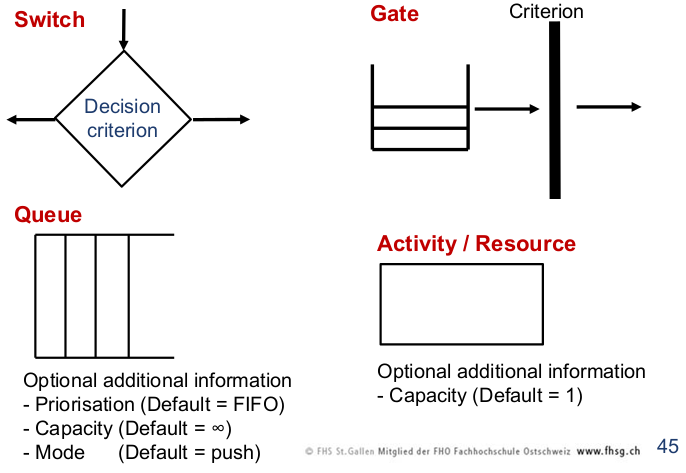
\includegraphics{figures/flowDiagramBuildingblocks1.png}
\caption{Building Blocks 1}
\end{figure}

\begin{figure}
\centering
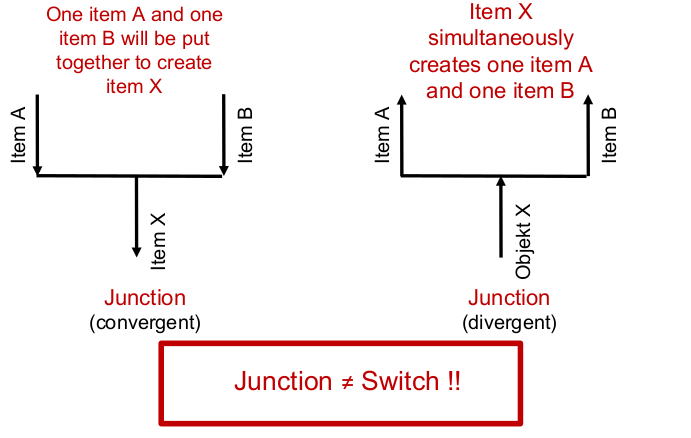
\includegraphics{figures/flowDiagramBuildingblocks2.png}
\caption{Building Blocks 2}
\end{figure}

\begin{figure}
\centering
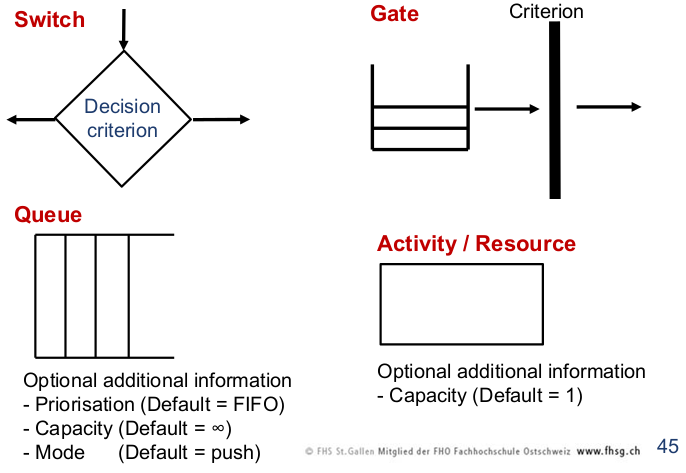
\includegraphics{figures/flowDiagramBuildingblocks1.png}
\caption{Building Blocks 3}
\end{figure}
